\section{Concrete implementation}
\label{sec:concrete}

\newcommand{\con}[1]{\ensuremath{{\color{red} #1}}}
\newcommand{\abs}[1]{\ensuremath{{\color{blue} #1}}}

The operational semantics we have defined in the previous section
satisfy termination sensitive non-interference by design.
We achieve this general statement that works for a large class of
languages by having different task execute completely isolated from
each other, such that every task has it's own state.
In some cases, this strong separation is desirable, or even necessary.
Languages like C provide direct access to the addresses without
mechanisms in the language to achieve a separation of the heap.
However, for other languages this isolation of tasks can be
undesirable, e.g., for performance reasons.
For instance, for the mini-ML language, our presentation so far
requires a separate heap per task, which is not very practical.
Instead, we would like to
more tightly couple the integration of the target and IFC
language by reusing existing infrastructure.  In the running example,
a concrete implementation might use a single global heap, and ensure
that references do not cross task boundaries, and thus preserving
non-interference.

In this section, we will detail an approach that allows one to implement
a concrete system guided conceptually by the ideas in the previous
section but making different choice for ease of implementation or
performance, and give conditions for when such a system preserves
non-interference.
We first explain the idea for the single heap mini-ML language, and then
generalize to arbitrary languages.

\subsection{IFC-Mini-ML with a Single Heap}

Instead of using a configuration of the form
\[|iconf iS (fullconf id1 il1 tS1 ie1, fullconf id2 il2 tS2 ie2 ldots)|\]
as is done in |specLangML alpha|
where every task has its
own ML heap, we would like a single global heap as in
|oneheapiconf iS tS (oneheapfullconf id1 il1 ie1, oneheapfullconf id2 il2 ie2, ldots)|.
To keep up a fictional separation between the portions
of the global heap that tasks can use, we forbid references to
cross task boundaries.  To achieve such a system, we can
adapt most of the operational rules easily to work with these
new configurations.  In the abstract system, the \textsc{I-fork}
rule created a fresh heap for the new task to execute in.  Since we
want to forbid references to cross task boundaries, we do not modify
the global heap and instead add an additional premise that the forked
expression |ie| must not contain any references.
Finally, we add the same condition to the \textsc{I-send} rule.
Tasks that try to fork or send an expression that contains a
reference will now get stuck, and will stop executing by the
\textsc{I-noStep} rule.
We call this family of languages |concreteLangMl alpha|, which
is still parametrized by the scheduling policy |alpha|.

\Red{Show the key rules here.}

In |concreteLangMl alpha| we
effectively restrict the abstract semantics in some cases (namely
to not allow the passing of references) as well as using a different
way to represent the heap.  How can we be sure that these
new, \textit{concrete semantics} for our system still satisfy
non-interference?

We will use two techniques to ensure non-interference.  First,
we require some form of isomorphism to the abstract language
|specLangML alpha| that ensures that the concrete system behaves
in a similar way.  Secondly, we pose conditions on what kind
of restrictions the concrete language is allowed to make
on the abstract language.

Intuitively, there are two scenarios in which non-interference
can be violated when restricting the transition relation:
\begin{itemize}
  \item Adding an additional premise to one of the rules that inspects
  information which is above the security label of the task currently
  executing.  This would allow another task to observe the termination
  of the other if both are at the same security level, and thus observe
  the secret information that was used in the additional
  premise of the rule.
  \item Adding additional restrictions to transition rules can
  also cause the whole configuration to get stuck, which can leak
  information through the termination channel (which is only
  of interest for TSNI, but not TINI, of course).
\end{itemize}

Next, we will make these two intuitions precise and give a general
definition for how non-interference can be preserved.  Then, we
show that the language |concreteLangMl alpha| satisfies these
conditions.

\Red{Should we give an example why removing transitions in general
  is not OK?  Edward has already typeset one that we could
  use.}

%This isn't trivial, as it is not sound to add arbitrary additional
%conditions on evaluation rules.  To see this, consider a contrived
%concrete system where we add a premise to a reduction rule that
%stops a task based on secret information.  Such a system will
%not satisfy non-interference, as it allows other tasks on the
%same level to observe the termination of that task and thus the
%secret information which was used to decide if the task terminates
%or not.

\subsection{Correctness of Concrete Semantics}

To formalize the conditions under which we can show the concrete
semantics preserve non-interference, we require some notation:

\begin{definition}[Weak isomorphism of information-flow control languages]
  A language \con{|(C, .->, erasef l)|} is \textit{weakly isomorphic} to a
  language \abs{|(iC, .->, erasef l)|} if there exist total functions
  |f : tC -> iC| and |finv : iC -> tC| such that |f .. finv = idf tC|
  |finv .. f = idf iC|.  Furthermore, the following coherence conditions
  must hold:
  \begin{itemize}
    \item |f| is functorial (e.g. if $\abs{x\ R\ y}$ then
    $f(\abs{x})\ \con{R}\ f(\abs{y})$) over both
    $l$-equivalences and |.->|, and
    \item |finv| is functorial over $l$-equivalence (though not necessarily |.->|).
  \end{itemize}
  We furthermore call the two languages \textit{isomorphic} if both
  |f| and |finv| are functorial over |.->|.
\end{definition}

Now, we can propose the following two-step process to ensure that
non-interference is preserved:
\Red{We should find a better name for this, or not use a name, or something.}
\begin{definition}[Non-interference preserving, restricted isomorphism (NPRI)]
  We call an IFC language
  |concreteLang alpha targetLang| (the concrete language for a given
  target language |targetLang| and scheduling policy |alpha|)
  a \textit{non-intereference preserving,
  restricted isomorphism} with regard to the IFC language
  |specLang alpha targetLang|
  (the abstract language) if the following
  two conditions hold:
  \begin{enumerate}
    \item Any of the reduction rules of the abstract
    semantics |specLang alpha targetLang|
    presented in Section~\ref{sec:retrofit} can
    be restricted by adding a predicate $P$ to the premise of
    any rule other than \textsc{I-noStep}.  The predicate $P$
    can depend only on the \textit{erased} configuration
    |erase il ic|, where |il| is the label of the first task
    in the task list and |ic| the full configuration.
    \item The concrete language
    |concreteLang alpha targetLang|
    must be isomorphic to the abstract semantics |specLang alpha targetLang|
    with the additional predicates $P$ on the rules.
  \end{enumerate}
\end{definition}

\begin{theorem}[NPRI implies non-interference]
  \label{thm:npri}
  If a language |concreteLang alpha targetLang| is a NPRI, and |alpha|
  is a scheduling policy that makes |specLang alpha targetLang| satisfy
  TINI or TSNI, then also
  |concreteLang alpha targetLang| satisfies TINI, or TSNI, respectively.
\end{theorem}

Before we give the proof of this theorem in Section~\ref{sec:proofs},
let's consider our single-heap ML-like IFC language and
show that it is in fact NPRI, and thus non-interfering.

\begin{theorem}
  The language |concreteLangMl alpha| is a NPRI.
\end{theorem}
As a trivial corollary, it follows that |concreteLangMl roundrobinf| is
TSNI, and |concreteLangMl seqf| is TINI.

\begin{proof}
  It is easy to see that condition (1) of NPRI is satisfied, since
  we only add a side condition to the rules \textsc{I-fork} and
  \textsc{I-send}, and the condition only inspects the expression
  of the current task, which is by the definition of |erasef il| not
  erased.
  
  This leaves us to give an isomorphism between |concreteLangMl alpha|
  and |concreteLang alpha targetLangMl|, which we do as follows.
  \Red{Actually give an isomorphism.}
\end{proof}


\subsection{Proof of Theorem~\ref{thm:npri}}
\label{sec:proofs}

Before we give the actual proof, we state and proof some properties
of isomorphisms.

\begin{theorem}[Weak isomorphism preserves termination insensitive non-interference]
  If a language \con{L} is included in a language \abs{L}, and \abs{L}
  satisfies TINI, then \con{L} satisfies TINI.
\end{theorem}

\begin{proof}
  Shown by transporting configurations and reduction derivations
  from \con{L} to \abs{L}, applying TINI and transporting the resulting
  equivalence back using functoriality of |finv| over $l$-equivalences.
\end{proof}

\begin{theorem}[Isomorphism preserves termination sensitive non-interference]
  If \ifc{L} is isomorphic to \tar{L} and \ifc{L} satisfies TSNI, then
  \tar{L} satisfies TSNI.
\end{theorem}

\begin{proof}
  Shown by transporting configurations and reduction derivations from
  \tar{L} to \ifc{L}, applying TSNI, and then transporting the
  resulting configuration, $l$-equivalence and multi-step derivation back.
\end{proof}

\Red{Adapt the following proofs.}

\begin{lemma}
  \label{lemma:tsni}
  For any configurations |ic1|, |ic1'|, |ic2|, and label |il| where
  \begin{equation} \label{eq:tsni-lemma-lhs}
  |ic1| \approx_{|il|} |ic2|
  \qquad \text{and} \qquad
  |ic1| |.->| |ic1'|
  \end{equation}
  then there exists a configuration |ic2'| such that
  \begin{equation} \label{eq:tsni-lemma-rhs}
  |ic1'| \approx_{|il|} |ic2'|
  \qquad \text{and} \qquad
  |ic2| |.->|^* |ic2'|
  \ \text{.}
  \end{equation}
\end{lemma}

\begin{proof}
  We proof the theorem by induction on the length of the derivation sequence in~\eqref{eq:tsni-lhs}.
  The base case for derivations
  of length 0 is trivial, allowing
  us to simple chose $|ic2'=ic2|$.  In the step case, we assume
  the theorem holds for derivation sequences of length up to $n$, and show that it also
  holds for those of length $n+1$.  We split the derivation sequence from~\eqref{eq:tsni-lhs} as follows:
  \[
  |ic1| |.->| |ic1''| |.->|^n |ic1'|
  \]
  for some configuration |ic1''|.  By Lemma~\ref{lemma:tsni}, we get
  |ic''| with
  \begin{equation} \label{eq:tsni-proof-1}
  |ic1''| \approx_{|il|} |ic2''|
  \qquad \text{and} \qquad
  |ic2| |.->|^* |ic2''|
  \end{equation}
  Applying the induction hypothesis to
  $|ic1''| |.->|^n |ic1'|$, we get |ic2'| with
  \begin{equation} \label{eq:tsni-proof-2}
  |ic1'| \approx_{|il|} |ic2'|
  \qquad \text{and} \qquad
  |ic2''| |.->|^* |ic2'|
  \end{equation}
  Stitching together the derivation sequences from~\eqref{eq:tsni-proof-1} and~\eqref{eq:tsni-proof-2} directly gives
  us~\eqref{eq:tsni-rhs}, which concludes the proof.
\end{proof}
\begin{proof}[Proof of Lemma~\ref{lemma:tsni}]
  We proof the lemma by induction on the derivation
  for~\eqref{eq:tsni-lemma-lhs}, and consider all possible rules that
  could have been used to make the reduction step.
  First, we observe there must be at least one task in |ic1|, otherwise
  it could not take a step.  Thus, |ic1| is of the form
  |iconf iS1 (it1, its1)|.  Consider two cases:
  \begin{itemize}
    \item $|erase il it1|=|bullet|$. In this case, we do not need to take a
    step for
    |ic2|, because |ic2'=ic2| will already be |il|-equivalent to |ic1'|.
    To see that, note that the tasks |its1| in |ic1| are left in the
    same order and unmodified. The task |it1| either
    gets dropped (by \textsc{I-noStep}), or
    transforms into a new task |it1'| as well as potentially spawning a new
    task |it1''|.  Since both |it1'| and |it1''| have a label that is
    at least as high as the label of |it1|, they will get filtered
    by |erasef il| in |ic1'|.
    Lets consider the possible changes to |iS1|: If |it1| sends a
    message, then the corresponding queue in |iS1'| will contain one
    more message.  However, that message has the label of |it1| (or a higher
    label), and will thus get erased by |erasef il|.
    Finally, receiving or not receiving a message (by
    \textsc{I-recv} or \textsc{I-noRecv}) only changes the queue of
    task |it1|, which are erased from |iS1|.
    This ensures that $|ic1'|\approx_{|il|}|ic2'|$.
    
    \alphacondition{We need all scheduling policies to not change the order
      of any tasks (except for the first one).  Newly spawned task can appear
      anywhere in the list.}
    \item $|erase il it1|\neq|bullet|$.  Here, there must be a corresponding
    task |it2| in |ic2|,
    such that |it1=it2| (otherwise |ic1| and
    |ic2| could not be |il| equivalent).
    However, |it2| might not be at the beginning of the task list yet, but
    all tasks occurring before it must get erased by |erasef il|.
    In |ic2|, we can first take some number of steps until |it2| moves
    to the front of the list (\Red{Say more precisely why
      (basically because we require the scheduling policy to do that)}).
    
    \alphacondition{The scheduling policy must eventually let any task in
      the task list evaluate.  In particular, it cannot get stuck when the
      first task gets stuck, or keep executing a small number of tasks
      exclusively forever (e.g. just execute the first task all the time
      if it gets into an infinite loop).}
    
    Therefore, after |ic2| has potentially executed some number of steps
    to arrive at |ic2''|, we are now in the situation where $|ic1|\approx_{|il|}|ic2''|$, and the first task |it1| and |it2| don't
    get erased and are thus equivalent.
    The task |it2| can now take exactly the same step as |it1|;  we only
    need to argue that the potential differences in |iS1| and |iS2| cannot
    have an influence on the execution (and we know |iS1| and |iS2| are
    |il| equivalent).
    Again, only send and receive will change |iS|, so we consider all
    rules that could have been used for~\eqref{eq:tsni-lemma-rhs}.  If
    a message is sent, then the message is added to the same queue.  This
    queue is either completely erased, or it is |il| equivalent.  In both
    cases, |il| equivalence of |iS1'| and |iS2'| is preserved.
    When the tasks are receiving a message, then by the reduction rules
    we know that they first filter the queue by the label of |it1|.  We
    also know that the queues are equivalent when filtered by the less
    restrictive label |il|, thus the messages received (or dropped) from the
    queue are equivalent.
  \end{itemize}
\end{proof}





\subsection{\Red{Previous Stuff (to be merged/removed as necessary)}}

The operational semantics we have derived in the previous section
constitutes an abstract \emph{specification}: a semantics for which
non-interference is (obviously) true.  This specification can guide the
design of an information-flow calculus which would not be directly
derivable from our procedure, but is related to some such derivation.
For example, in our mini-ML language, the combined semantics requires
each thread to have a separate ML heap.  In an actual implementation, we
might like to only have a single heap and disallow the passing of
references between threads.  This restriction maintains a correspondence
between the abstract multiple heaps and the concrete single heap.  We might
hope that we can prove noninterference for this new system by reusing
noninterference for the old system.

However, modifying operational rules poses a distinct problem for
preserving non-interference.  Consider a trivial state machine as shown
in Figure~\ref{fig:trivial-sm}, whose second projection is classified
secret.  With all three transitions, this language fulfills
termination-sensitive noninterference.  Furthermore, if the dashed line
is removed, the language continues to satisfy TSNI.  However, if any
solid line is removed, however, the language fails TSNI.

\begin{figure}
    States: $(x,y)$ for $x,y \in \{0,1\}$ \\
    Erasure function: $f(x,y) = (x,\bullet)$

    \begin{center}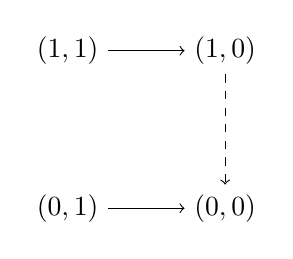
\begin{tikzpicture}[node distance=2cm, auto]
        \node (A) {$(1,1)$};
        \node (B) [right of=A] {$(1,0)$};
        \node (C) [below of=A] {$(0,1)$};
        \node (D) [right of=C] {$(0,0)$};
        \draw[->] (A) to node {} (B);
        \draw[->] (C) to node {} (D);
        \draw[->, dashed] (B) to node {} (D);
    \end{tikzpicture}\end{center}

    \label{fig:trivial-sm}
    \caption{A trivial state machine}
\end{figure}

The approach we will take is in two steps.  First, we sidestep the
restriction problem by demanding that the concrete implementation be
\emph{isomorphic} to the abstract specification, but perhaps having a different
runtime representation (a single heap) and some well-formedness
condition (every item on the heap only contains pointers from a single
location).  Isomorphism will preserve nonintereference, but it will also means all
transitions in the abstract language have to be implemented, including
undesirable transitions such as sending a pointer to another thread makes
the pointer dangling.  Next, we define a desugaring into this language
which adds dynamic checks, eliminating the possibility for these undesirable
transitions to be exercised.


Before we show isomorphism preserves termination sensitive
non-interference, we'd like to remark that one can safely remove transitions
and preserve termination \emph{insensitive} interference:


\begin{figure}

\begin{mathpar}
\inferrule[I-stepT]
{|
conf tS (te) -> conf tS' te'
|}
{|
coconf iS tS (cconf id il (iniE (IT te)), ldots)
.->
iS ; tS' ; sched step (cconf id il (iniE (IT te')), ldots)
|}

\and
% This rule is not complete, needs the FV condition
\inferrule[C-fork]
{ 
|iS' = iS [ id' mapsto nil ]|\\
|it1 = cconf id il (iniE id')|\\
|itnew = cconf id' il (TI ie)|\\
|fresh (id')|
}
{|
coconf iS tS (lconf id il (iniE (fork ie)), ldots)
.->
iS'; tS; sched fork (it1, ldots, itnew)
|}
\end{mathpar}

\caption{ML with a single heap}
\label{fig:comb}
\end{figure}

